\documentclass[
	a4paper,
	oneside,
	BCOR = 10mm,
	DIV = 12,
	12pt,
	headings = normal,
]{scrartcl}

%%% Length calculations
\usepackage{calc}
%%%

%%% Support for color
\usepackage{xcolor}
\definecolor{lightblue}{HTML}{03A9F4}
\definecolor{red}{HTML}{F44336}
%%%

%%% Including graphics
\usepackage{graphicx}
%%%

%%% Font selection
\usepackage{fontspec}

\setromanfont{STIX Two Text}[
	SmallCapsFeatures = {LetterSpace = 8},
]

\setsansfont{IBM Plex Sans}[
	Scale = MatchUppercase,
]

\setmonofont{IBM Plex Mono}[
	Scale = MatchUppercase,
]
%%%

%%% Math typesetting
\usepackage{amsmath}

\usepackage{unicode-math}
\setmathfont{STIX Two Math}

\usepackage{IEEEtrantools}
%%%

%%% List settings
\usepackage{enumitem}
\setlist[enumerate]{
	label*      = {\arabic*.},
	leftmargin  = *,
	labelindent = \parindent,
	topsep      = 1\baselineskip,
	parsep      = 0\baselineskip,
	itemsep     = 1\baselineskip,
	noitemsep, % override itemsep
}

\setlist[itemize]{
	label*      = {—},
	leftmargin  = *,
	labelindent = \parindent,
	topsep      = 1\baselineskip,
	parsep      = 0\baselineskip,
	itemsep     = 1\baselineskip,
	noitemsep, % override itemsep
}

\setlist[description]{
	font        = {\rmfamily\upshape\bfseries},
	topsep      = 1\baselineskip,
	parsep      = 0\baselineskip,
	itemsep     = 0\baselineskip,
}

%%%

%%% Structural elements typesetting
\setkomafont{pagenumber}{\rmfamily\upshape}
\setkomafont{disposition}{\rmfamily\bfseries}

% Sectioning
\RedeclareSectionCommand[
	beforeskip = -1\baselineskip,
	afterskip  = 1\baselineskip,
	font       = {\normalsize\bfseries\scshape},
]{section}

\RedeclareSectionCommand[
	beforeskip = -1\baselineskip,
	afterskip  = 1\baselineskip,
	font       = {\normalsize\bfseries\itshape},
]{subsection}

\RedeclareSectionCommand[
	beforeskip = -1\baselineskip,
	afterskip  = 1\baselineskip,
	font       = {\normalsize\bfseries},
]{subsubsection}

\RedeclareSectionCommand[
	beforeskip = -1\baselineskip,
	afterskip  = -0.5em,
	font       = {\normalsize\mdseries\scshape\addfontfeatures{Letters = {UppercaseSmallCaps}}},
]{paragraph}
%%%

%%% Typographic enhancements
\usepackage{microtype}
%%%

%%% Language-specific settings
\usepackage{polyglossia}
\setmainlanguage{ukrainian}
\setotherlanguages{english}
%%%

%%% Captions
\usepackage{caption}
\usepackage{subcaption}

%\DeclareCaptionLabelFormat{closing}{#2)}
%\captionsetup[subtable]{labelformat = closing}

%\captionsetup[subfigure]{labelformat = closing}

\captionsetup[table]{
	aboveskip = 0\baselineskip,
	belowskip = 0\baselineskip,
}

\captionsetup[figure]{
	aboveskip = 1\baselineskip,
	belowskip = 0\baselineskip,
}

\captionsetup[subfigure]{
	labelformat = simple,
	labelformat = brace,
}
%%%

%%% Hyphenated ragged typesetting
\usepackage{ragged2e}
%%%

%%% Table typesetting
\usepackage{booktabs}
\usepackage{longtable}

\usepackage{multirow}

\usepackage{array}
\newcolumntype{v}[1]{>{\RaggedRight\arraybackslash\hspace{0pt}}p{#1}}
\newcolumntype{b}[1]{>{\Centering\arraybackslash\hspace{0pt}}p{#1}}
\newcolumntype{n}[1]{>{\RaggedLeft\arraybackslash\hspace{0pt}}p{#1}}
%%%

%%% Drawing
\usepackage{tikz}
\usepackage{tikzscale}
\usetikzlibrary{positioning}
\usetikzlibrary{arrows.meta} % Stealth arrow tips
%%%

%%% SI units typesetting
\usepackage{siunitx}
\sisetup{
	output-decimal-marker = {,},
	exponent-product      = {\cdot},
	inter-unit-product    = \ensuremath{{} \cdot {}},
	per-mode              = symbol,
}
%%%

%%% Framing code listings
\usepackage{tcolorbox}
\tcbuselibrary{breakable}
\tcbuselibrary{minted}
\tcbuselibrary{skins}

\newtcblisting[
	auto counter, 
	list inside, 
	number within = section,
]{listingpython}[3][]{%
	minted language = python,
	minted style    = bw,
	minted options  = {
		linenos,
		tabsize = 4,
		breaklines,
		% breakanywhere,
		fontsize = \footnotesize,
		autogobble
	},
	%
	% empty,
	sharp corners,
	colframe         = black,
	colback          = black!0,
	leftrule         = 0em,
	rightrule        = 0em,
	toprule          = 1pt, % orig = 0pt
	bottomrule       = 1pt, % orig = 0pt
	titlerule        = 0.5pt,
	colbacktitle     = black!0,
	coltitle         = black,
	toptitle         = 0.3em,
	bottomtitle      = 0.1em,
	borderline north = {1pt}{0pt}{black},
	borderline south = {1pt}{0pt}{black},
	before skip      = \intextsep,
	after  skip      = \intextsep,
	title            = {Лістинг \thetcbcounter: #2},
	list entry       = {\protect\numberline{\thetcbcounter}#2},
	left = 0em,
	right = 0em,
	%
	listing only,
	breakable,
	%
	label = {#3},
	%
	#1
}

\newtcbinputlisting[auto counter, list inside, number within = section]{\inputpython}[4][]{%
	minted language = python,
	minted style    = bw,
	minted options  = {
		linenos,
		tabsize = 4,
		breaklines,
		breakbytokenanywhere,
		fontsize = \footnotesize,
	},
	%
	% empty,
	sharp corners,
	colframe         = black,
	colback          = black!0,
	leftrule         = 0em,
	rightrule        = 0em,
	toprule          = 0pt, % orig = 0pt
	bottomrule       = 0pt, % orig = 0pt
	titlerule        = 0.5pt,
	colbacktitle     = black!0,
	coltitle         = black,
	toptitle         = 0.3em,
	bottomtitle      = 0.1em,
	borderline north = {1pt}{0pt}{black},
	borderline south = {1pt}{0pt}{black},
	before skip      = \intextsep,
	after  skip      = \intextsep,
	title            = {Лістинг \thetcbcounter: #3},
	list entry       = {\protect\numberline{\thetcbcounter}#3},
	left = 0em,
	right = 0em,
	%
	listing file={#2},
	listing only,
	breakable,
	%
	label = {#4},
	%
	#1
}

% Customize minted
\usepackage{minted}
\setmintedinline{
	style = bw,
	breaklines,
}

% Customize minted line numbers
\renewcommand{\theFancyVerbLine}{\ttfamily\scriptsize\arabic{FancyVerbLine}}

%%%

%%% Links and hyperreferences
\usepackage{hyperref}
\hypersetup{
	bookmarksnumbered = true,
	colorlinks      = false,
	linkbordercolor = red,
	urlbordercolor  = lightblue,
	pdfborderstyle  = {/S/U/W 1.5},
}
%%%

%%% Length adjustments
% Set baselineskip, default is 14.5 pt
\linespread{1.068966} % ~15.5 pt
\setlength{\emergencystretch}{1em}
\setlength{\parindent}{1.5em}
\newlength{\gridunitwidth}
\setlength{\gridunitwidth}{\textwidth / 12}
%%%

%%% Custom commands
\newcommand{\allcaps}[1]{{\addfontfeatures{LetterSpace = 8, Kerning = Off}#1}}
\newcommand{\filename}[1]{\texttt{#1}}
\newcommand{\progname}[1]{\texttt{#1}}
\newcommand{\modulename}[1]{\texttt{#1}}
%%%

%%% Custom math commands
\newcommand{\longvar}[1]{\mathit{#1}}
%%%

\begin{document}

\begin{titlepage}
		\begin{center}
			Міністерство освіти і науки України\\
			Національний авіаційний університет\\
			Навчально-науковий інститут комп'ютерних інформаційних технологій\\
			Кафедра комп'ютеризованих систем управління

			\vspace{\fill}
				Лабораторна робота №3\\
				з~дисципліни «Імітаційне моделювання»\\
				на~тему «Моделювання дискретних випадкових величин»\\

			\vspace{\fill}

			\begin{flushright}
				Виконав:\\
				студент \allcaps{ННІКІТ}\\
				групи СП-325\\
				Клокун В.\,Д.\\
				Перевірила:\\
				Марченко Н.\,Б.
			\end{flushright}

			Київ 2019
		\end{center}
	\end{titlepage}

	\section{Мета роботи}
		Ознайомитись з~алгоритмом побудови ряду розподілу дискретних випадкових величин та його графічним зображенням; побудувати імітаційну модель отримання системи дискретних випадкових величин.

	\section{Хід роботи}
		\paragraph{Завдання} В партії з~$n_1$ деталей є~$n_2$ стандартних деталей. Навмання з усієї партії вибирається 2~деталі. Побудувати ряд розподілу числа~$X$~— числа стандартних деталей серед відібраних. Скористатись гіпергеометричним розподілом.

		Під час виконання роботи була розроблена імітаційна модель для виконання поставлених завдань і реалізована у вигляді відповідного програмного засобу (ліст.~\ref{lst:full-solution}). Реалізований програмний засіб був запущений на~моделювання і~надавав стабільний і~очікуваний результат~(рис.~\ref{fig:program_scr}).

		\begin{figure}[!htbp]
			\centering
			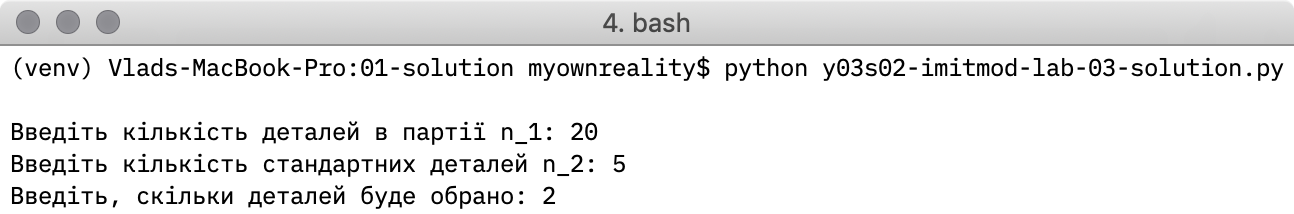
\includegraphics[height = 4\baselineskip]{./assets/y03s02-imitmod-lab-03-p00.png}
			\caption{Результат роботи програми: вікно терміналу}
			\label{fig:program_scr}
		\end{figure}

		В результаті роботи програма будує ряд розподілу числа~$X$ у~вигляді графіку функції ймовірностей~(рис.~\ref{subfig:pmf}), а~також многокутник розподілу~(рис.~\ref{subfig:dist-polygon}).

		\begin{figure}[!htbp]
			\centering
			\begin{subfigure}[t]{0.5\columnwidth}
				\centering
				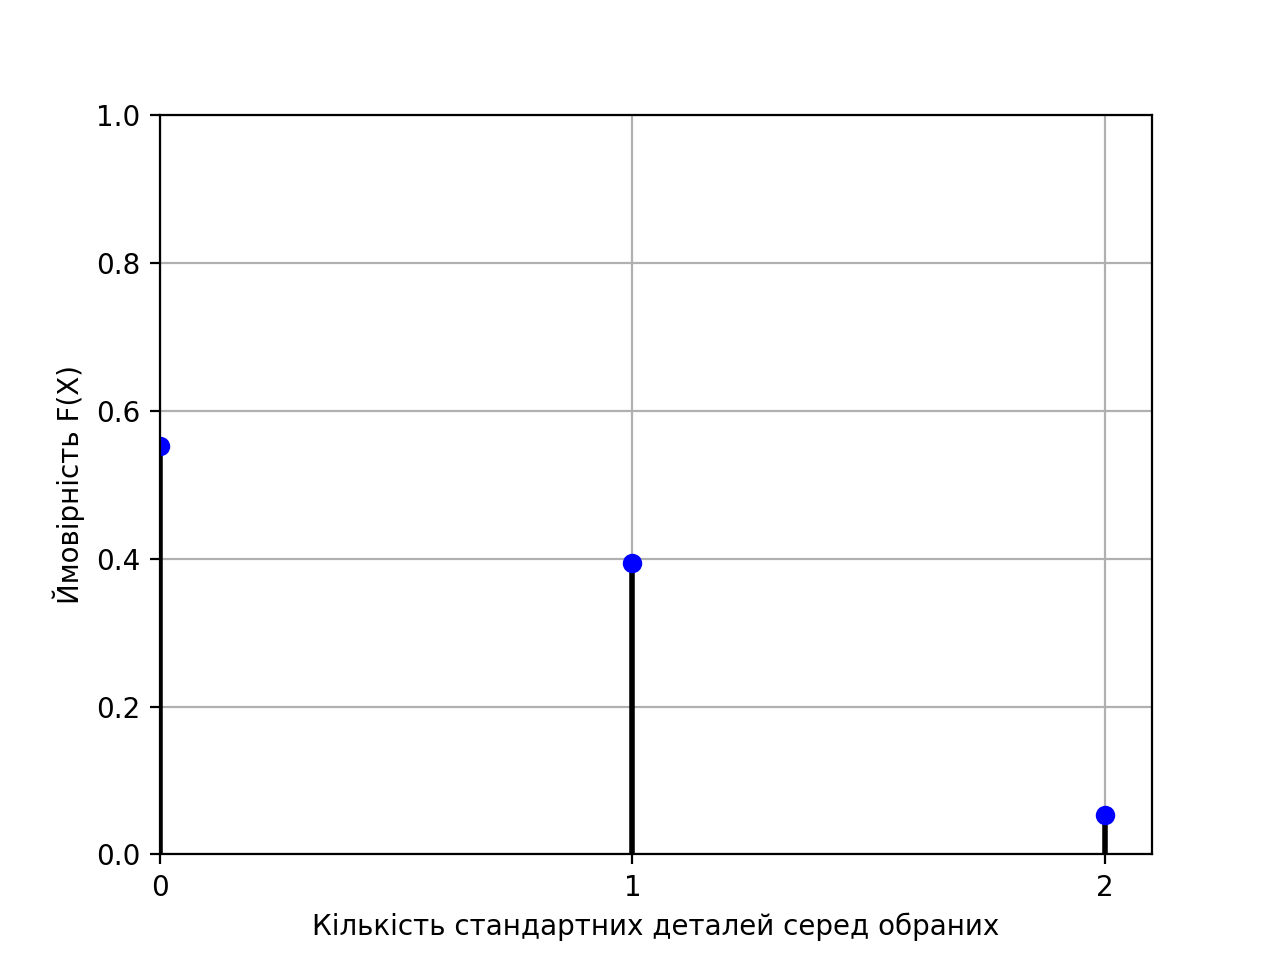
\includegraphics[width = \columnwidth]{./assets/y03s02-imitmod-lab-03-p01.png}
				\caption{}
				\label{subfig:pmf}
			\end{subfigure}%
			\begin{subfigure}[t]{0.5\columnwidth}
				\centering
				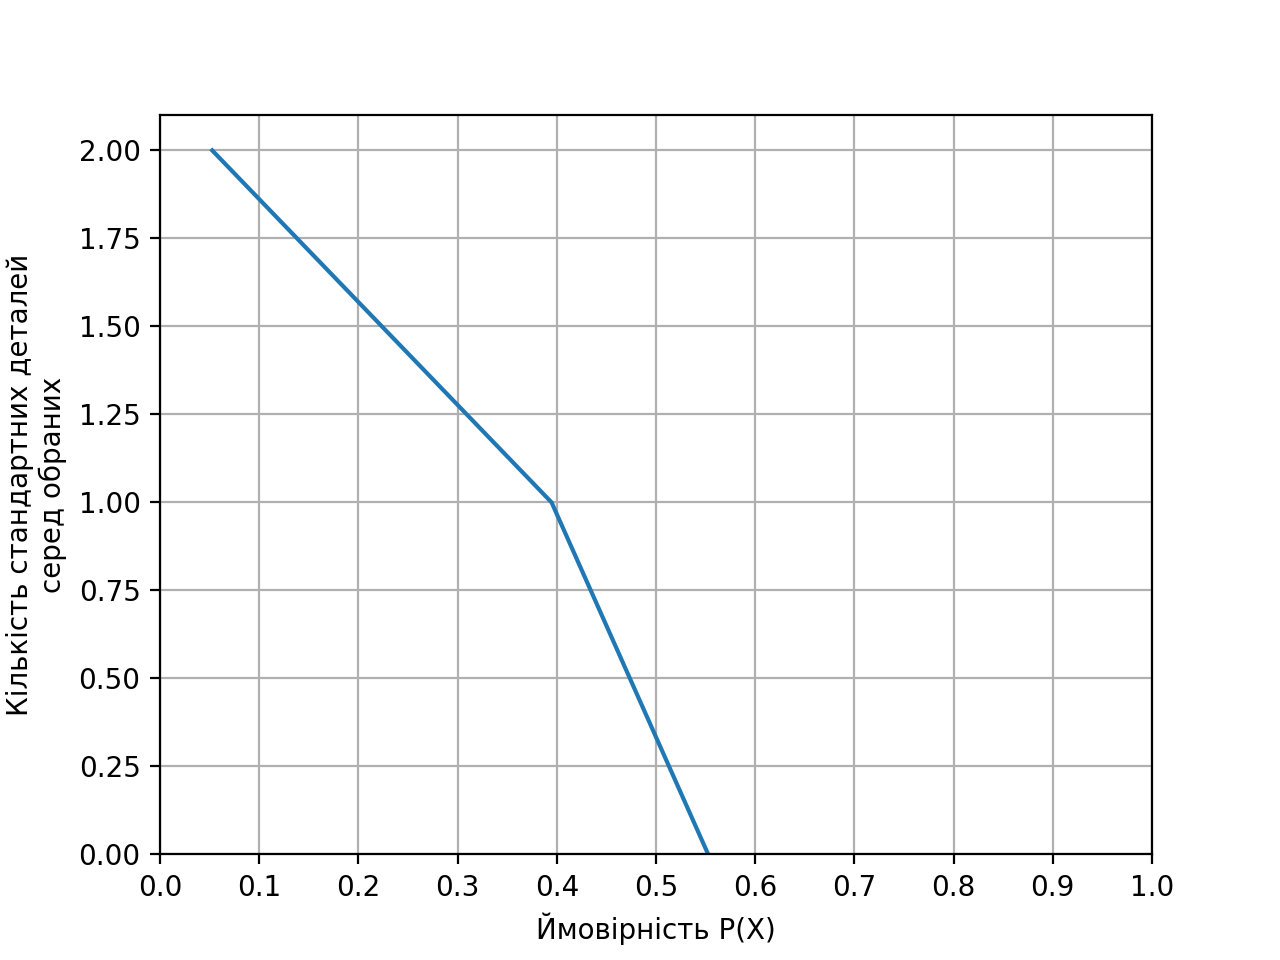
\includegraphics[width = \columnwidth]{./assets/y03s02-imitmod-lab-03-p02.png}
				\caption{}
				\label{subfig:dist-polygon}
			\end{subfigure}
			\caption{Графіки, створені програмою: \subref{subfig:pmf}~— графік розподіл ймовірностей, \subref{subfig:dist-polygon}~— многокутник розподілу}
			\label{fig:plots}
		\end{figure}

		\section{Висновок}
			Виконуючи дану лабораторну роботу, ми ознайомились з~алгоритмами моделювання результатів випробувань випадкових подій; побудували імітаційну модель функціонування системи протягом деякого часу.

		\appendix
		\section{Повний початковий код програмної реалізації}
		\label{sec:full-listing}
			\begin{listingpython}[toprule = 0pt, bottomrule = 0pt]{Повний початковий код програмної реалізації}{lst:full-solution}
import numpy as np
import scipy.stats as sp_stats
import matplotlib.pyplot as plt


def split_list_of_points(lofp):
    lx, ly = zip(*lofp)
    return lx, ly


def main():
    n_1 = float(input('Введіть кількість деталей в партії n_1: '))
    n_2 = float(input('Введіть кількість стандартних деталей n_2: '))
    num_samples = float(input(('Введіть, скільки деталей буде обрано: ')))

    total = n_1  # Total number of outcomes
    good = n_2   # Number of good outcomes

    rand_var = sp_stats.hypergeom(total, good, num_samples)
    possible_outcomes = np.arange(num_samples+1)
    # pmf --- probability mass function
    pmf_details = rand_var.pmf(possible_outcomes)

    # Probability function
    fig = plt.figure(1)

    ax = fig.add_subplot(111)
    ax.plot(possible_outcomes, pmf_details, 'bo')
    # Plot vlines from 0 to the probability value
    ax.vlines(possible_outcomes, 0, pmf_details, lw=2)
    ax.set_xticks(possible_outcomes)
    ax.set_xlim(0.0, None)
    ax.set_ylim(0.0, 1.0)
    ax.set_xlabel('Кількість стандартних деталей серед обраних')
    ax.set_ylabel('Ймовірність F(X)')
    plt.grid()

    # Probability distribution polygon
    fig = plt.figure(2)
    plt.subplot(111)
    ax = fig.add_subplot(111)
    # Create a list of graph points sorted by X value (pmf_details)
    points = [i for i in sorted(zip(pmf_details, possible_outcomes))]
    # Split a list of points into tuples of X and Y coordinates
    x, y = split_list_of_points(points)
    ax.plot(x, y)
    ax.set_xlim([0.0, None])
    ax.set_ylim([0.0, None])
    ax.set_xticks(np.arange(1.1, step=0.1))
    ax.set_xlabel('Ймовірність P(X)')
    ax.set_ylabel('Кількість стандартних деталей\nсеред обраних')

    plt.grid()
    plt.show()


if __name__ == '__main__':
    main()
			\end{listingpython}

\end{document}

